\chapter{Implementation}
\label{ch:Implementation}

In this chapter, we deduce the necessary equations to implement the reduction algorithm.
We focus on summation, our reduction operator $\reduce$ is the simple floating-point addition.
While the recursive formula given in \Cref{eq:nodeReduceReduction} already defines a reduction algorithm, its implementation in imperative languages would heavily rely on the call stack to store subtotals.
In practice, performing the calculations in opposite direction, bottom-up instead of than top-down, yields better runtimes.

The bionary representation of element indices has $\numLevels$ digits, since
\begin{equation}
2^{\numLevels} \geq 2^{\log_2 N} = N
\end{equation}
If we interpret the digits of an index ordered from most to least significant as a series of decisions where $0$ means \enquote{go up}
and $1$ means \enquote{go right and up}, each index encodes a path from the tree root to the corresponding leaf node:

\begin{figure}[H]
\centering
\begin{tikzpicture}
\newcommand{\heightFactor}{0.7}
\newcommand{\treeN}{8}
\newcommand{\subtreeHeight}[2]{\directlua{tex.write(subtree_height(#1,#2))}}
\newcommand{\parentIdx}[1]{\directlua{tex.write(parent(#1))}}
\foreach \x in {0,...,\treeN} {
	\node [anchor=south] (idx\x{}) at (\x{},0) {\x};
	
	\draw (\x{},0)
		-- (\x{},-\heightFactor * \subtreeHeight{\x}{\treeN}-\heightFactor)
		-- (\parentIdx{\x},-\heightFactor * \subtreeHeight{\x}{\treeN}-\heightFactor);
}

% Highlighted path
\draw [very thick,red] (6,0) -- (6, -2 * \heightFactor) -- (4, -2 * \heightFactor) -- (4, -3*\heightFactor) -- (0, -3*\heightFactor) -- (0,-5*\heightFactor);
\node [red] at (0-0.3, -3.5*\heightFactor) {0};
\node [red] at (2, -2.5*\heightFactor) {1};
\node [red] at (5, -1.5*\heightFactor) {1};
\node [red] at (6-0.3, -0.5*\heightFactor) {0};

\draw [->,red] (-0.3,-\heightFactor * \subtreeHeight{0}{\treeN}-\heightFactor + 0.1) -- +(0,0.3);

\node at (10,-2) {$6_{10} = 0110_2$};
\end{tikzpicture}
\caption{Example path for index $6$ with $N = 10$}
\label{fig:indexTreePath}
\end{figure}

For any given $x$-coordinate ($x > 0$), the \textbf{maximum $y$-coordinate} $\max_y(x)$ is equal to the position of the first (least significant) bit set in $x$, minus 1; this corresponds to the number of trailing zeros.
We denote this expression as $\ffs (x) - 1$.
The term $\ffs$ stems from the eponymous function of the C library \texttt{strings.h}.
The path representation explains why the equality holds: the least significant bit is the last time the $x$-coordinate has changed, since all trailing zeros encode the decision \enquote{go up}.

To find the coordinates of the \textbf{parent node} of an inner node $(x, \max_x(y))$, we replace the last (least-significant) \enquote{go right and up} decision with \enquote{go up}. 
Numerically, this is equivalent to cancelling the least significant bit of $x$.
The expression $x \BitAnd (x - 1)$, where $'\BitAnd'$ is the bitwise AND-operation, is an efficient implementation of this operation.
Thus, we obtain the following definition of the parent function:

\begin{equation}
\label{eq:parent}
\textrm{parent} (x, \max_x (y) ) := (x \BitAnd (x - 1), y + 1)
\end{equation}

Each \gls{pe} with rank $i$ (where $i \in [0, P - 1]$) stores $n_i$ consecutive elements.
The global index of the first element assigned to a \gls{pe} is the so-called start index, and it is equal to the prefix sums of the assigned number of summands:

\begin{align}
\textrm{startIndex} (0) &= 0 \\
\textrm{startIndex} (i) &= \sum_{j = 0}^{i - 1} n_i
\label{eq:startIndex}
\end{align}

This allows us to define the function rankFromIndex, which computes the index of a \gls{pe} that stores a given summand:
\begin{equation}
\textrm{rankFromIndex} (x) = \max \{i \in [0, P - 1] \;|\; \textrm{startIndex} (i) \leq x \}
\end{equation}

The definition of the set of \gls{pe}-intersecting summand indices also depends on the rankFromIndex function:

\newcommand{\rankIntersectingIndices}{I_{\textrm{\gls{pe}-intersecting}}}
\begin{equation}
\rankIntersectingIndices (I) = \{i \in I \;|\; \textrm{rankFromIndex} (i) \neq \textrm{rankFromIndex} (\textrm{parent} (i)) \}
\end{equation}

\begin{algorithm}
\caption{Summation procedure}\label{algo:SummationAlgo}
\DontPrintSemicolon
\SetAlgoLined
$startIndex \gets startIndices (rank)$\;
$endIndex \gets startIndex + n_{\textrm{rank}}$\;
\For{$i \gets \rankIntersectingIndices ([\textrm{startIndex}, \textrm{endIndex}]) $}{
	\For{$y \gets [1, \max_x(y)]$}{
		$x \gets startIndex$\;
		\While{$x < endIndex$}{
			$a \gets (x, y - 1)$\;
			$indexB \gets x + 2^{y - 1}$\;
			\uIf{$indexB \geq N$} {
				$(x,y) \gets a$\;
			}
			\uElseIf{$\textrm{rankFromIndex}(indexB) \neq rank$}{
				$b \gets \textrm{fetch}\ indexB$\;
				$(x,y) \gets a + b$\;
			}
			\Else{
				$b \gets (indexB, y-1)$\;
				$(x,y) \gets a + b$\;
			}
			$x \gets x + 2^{y - 1}$\;
		}
	}
}
\end{algorithm}

\Cref{algo:SummationAlgo} shows to complete procedure that each \gls{pe} follows.
It consists of three nested loops.
The most outer loop iterates over all \gls{pe}-intersecting indices in ascending order.
The next loop implements the bottom-up scheme that was discussed at the beginning of this chapter, the $y$-values are incremented with each iteration.
Finally, the inner loop iterates over values of $x$ and sums up adjacent nodes.
There is some logic necessary to avoid out-of-bounds memory access ($indexB \geq N$) and deal with \gls{pe}-boundaries ($rankFromIndex(indexB) \neq rank$).

\section{Applied Optimizations}
\label{sec:AppliedOptimizations}

\subsection{Message Buffering}
\label{sec:MessageBuffering}

Depending on the distribution of summands, the first few \gls{pe}-intersecting nodes may have the same parent \gls{pe}. In these cases, the communication
overhead outweighs the actual computational effort of summation and bundling messages results in performance gains. The current implementation
utilizes a buffer with a maximum of $4$ summands per message. After the summation routine has computed a \gls{pe}-intersecting subtotal, it is placed
in a outbound message buffer. Flushing of the buffer occurs in either one of the following cases: \begin{itemize}
\item The summation routine inserts another \gls{pe}-intersecting summand into the buffer which has a different target \gls{pe}
\item The summation routine begins work on a subtotal whose subtree size is greater than $64$ summands
\end{itemize}

The buffer utilization averages about $1.2$ summands per message, further tests have shown that relaxing above flushing criteria does not
yield a runtime benefit, presumably because of the induced latency.

\subsection{Data Distribution}
\label{sec:DataDistribution}

If the user is in control of the summand distribution, multiple optimization techniques arise. To quantify them, we propose the following model:

\begin{equation}
\label{eq:distributionScore}
\textrm{Score} = t_{\textrm{MPI\_Send}} * n_{\textrm{\gls{pe} Intersecting Numbers}} + \max \{ i \in [0, p - 1]\, |\, n_i * t_{\textrm{add}} \}
\end{equation}

$t_{\textrm{MPI\_Send}}$ and $t_\textrm{add}$ are estimates of the time needed to send a single summand between two \glspl{pe} and addition of two
floating-point values with double precision (64 bit) respectively. On the shared-memory machine \textit{i10pc138}\footnote{See Appendix for hardware specifications}, these
estimates were empirically measured to be $t_{\textrm{MPI\_Send}} \approx 281ns$ and $t_\textrm{add} \approx 4.15ns$. While this model does not
take any data dependencies between subtotals into account, it balances the performance gain achieved by parallelization (represented by a low maximum
on the right side of \Cref{eq:distributionScore} against the communication overhead caused by binary tree fragmentation. 

In this section we will evaluate multiple approaches to the optimization of the data distribution with an example dataset with $N = 504\,850$ summands
and $p = 256$ \glspl{pe}.


\subsubsection{Even distribution}
This is the base case where each \gls{pe} has the same number of summands. If the total number of summands $N$ is not divisible by the number of
\glspl{pe}, the remainder will be put on the \glspl{pe} with the highest rank:

\begin{equation}
\label{eq:evenDistribution}
n_i (N, p) = \begin{cases}
\lfloor \tfrac{N}{p} \rfloor & i < N - N \bmod p \\
\lfloor \tfrac{N}{p} \rfloor + 1 & \textrm{otherwise}
\end{cases}
\end{equation}

In our model, the even distribution ensures maximal parallelization of the computational effort, since the maximum difference in the workload of a
\gls{pe} is $1$. With our test dataset, $1401$ messages are necessary, a score that can easily be bested.

\subsubsection{Round down to power of 2}
\label{sec:roundDownPower2Distribution}
Since most messages are caused by \gls{pe}-boundaries that cut the binary tree at \enquote{inconvenient} places, in a first attempt of data distribution
optimization we round down the number of assigned summands down to the nearest power of $2$,
the reasoning being that powers of $2$ have a lot of trailing
zeros and start indices with a lot of trailing zeros produce larger \gls{pe}-local subtrees, thus reducing the need for outbound messages.

\begin{equation}
\label{eq:roundDownPower2Distribution}
n_i (N, p) = \begin{cases}
2^{\lfloor \log_2 \frac{N}{p} \rfloor} & i < p - 1\\
N - \sum_{i=0}^{p-2} n_i (N,p) & i = p - 1
\end{cases}
\end{equation}

The rounding decreases the amount of messages considerably. With our test dataset, the message count is in the vicinity of the lower bound of $p - 1$, only
256 messages are needed, $20\%$ compared to the even distribution. This comes at the cost of an unbalanced summand distribution, the \gls{pe}
with the highest rank, where the remaining summands are stored, contains almost half the summands.
The inefficient parallelization is penalized with the second term of our score function, causing the score to be $2.7\times$ higher compared to
the even distribution.

\subsubsection{Optimized-Index Distribution}
As seen in the previous \Cref{sec:roundDownPower2Distribution}, unbounded distribution optimization yields small message counts at the expense of computational imbalance.
In this section we will present a method to optimize the data distribution within certain bounds, to balance communication and computational costs.

First, let $I_\textrm{start}(i)$ be a function that maps a \gls{pe}-index $i$ to the index of the first summand located on that \gls{pe}:

\begin{align}
\label{eq:startIndexDefinition}
I_\textrm{start}(0) &= 0 \\
I_\textrm{start}(i) &= \sum_{j=0}^{i - 1} n_i
\end{align}

Furthermore, let $\textrm{fairShare} = \tfrac{N}{p}$ be the average number of summands per \gls{pe} in an equivalent even distribution. We want to optimize each $I_\textrm{start}$ to cut off the least amount of edges while maintaining a fairly even distribution. This requirement can be expressed as follows:
\begin{equation}
\label{eq:optimizedIndexBounds}
\forall i \in \{1, \ldots, p - 1\}: I_\textrm{start}(i) - I'_\textrm{start}(i) \leq \alpha * \textrm{fairShare}
\end{equation}
where $I'_\textrm{start}$ is our optimized start index and $\alpha$ is the maximum deviation relative to the even distribution.
We now can iteratively improve our start index by applying the parent function \ref{eq:parent} until we are about to exceed the predefined bounds:

\begin{algorithm}
\caption{Index optimization procedure}\label{algo:optimizeIndex}
\DontPrintSemicolon
\SetAlgoLined
\SetKwInOut{Input}{input}

\Input{\gls{pe}-index $i$, start index $j$, maximum deviation parameter $\alpha$}

$currentIndex = j$\;
$proposedIndex = currentIndex$\;

\While{$\textrm{initialIndex} - \textrm{proposedIndex} \leq \alpha * \tfrac{N}{p}$} {
	$currentIndex = proposedIndex$\;
	$proposedIndex = parent(initialIndex)$\;
}
\end{algorithm}

After hand-tuning the parameter $\alpha = 0.0005$ with $N = 239 763$, $p = 256$ the runtimes measured over $40 000$ repetitions are plotted in \Cref{fig:distribution_runtimes}.
The runtime benefit is clearly visible, the optimized distribution is about $4µs$ faster than the even distribution.

\begin{figure}
\centering
\includegraphics[scale=0.75]{figures/distribution_experiment}
\caption{Runtime comparison of unoptimized vs.\ optimized data distribution}
\label{fig:distribution_runtimes}
\end{figure}


\subsection{Index-lookup Hashmap}
\label{sec:IndexLookupHashmap}

\begin{figure}
\centering
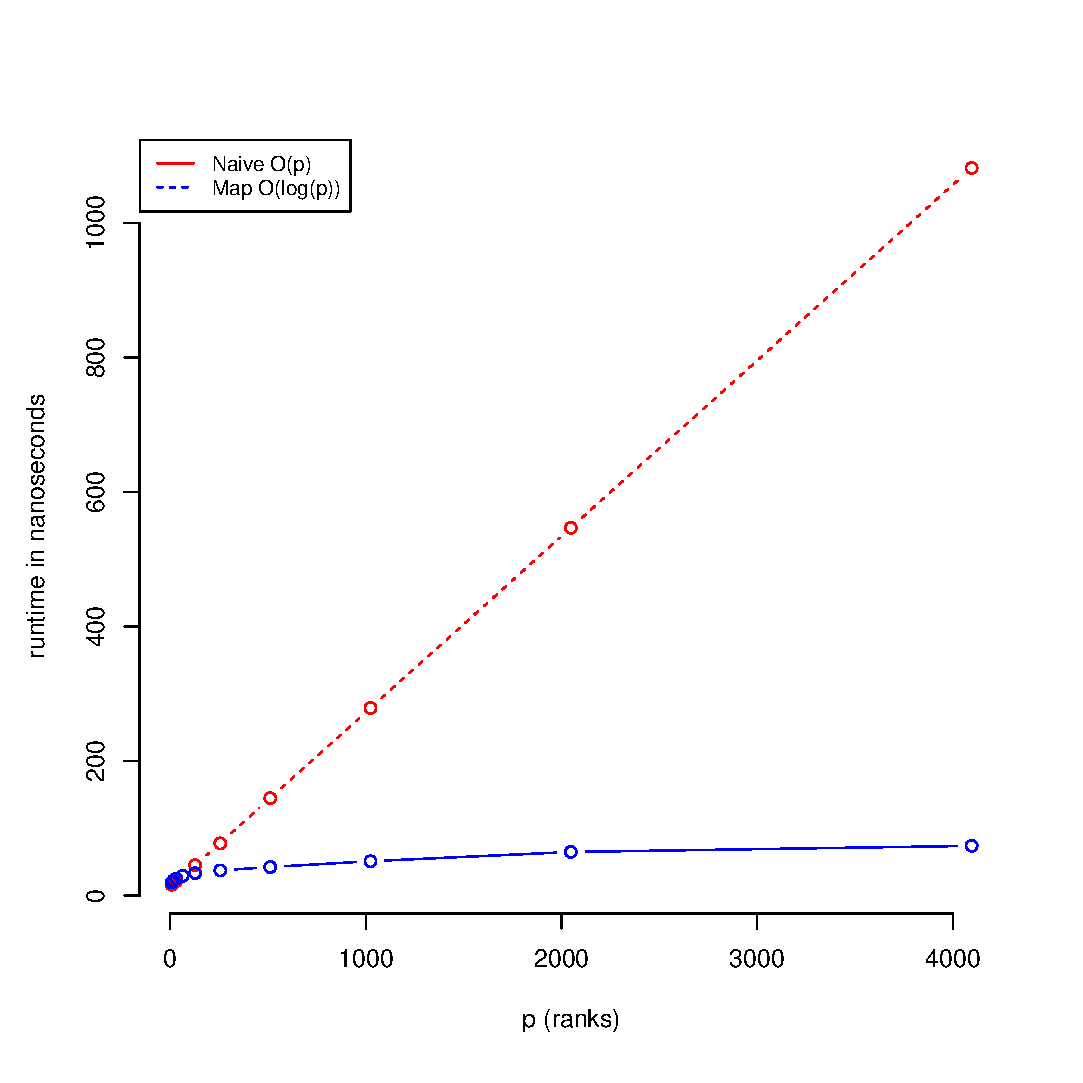
\includegraphics[scale=0.55]{figures/microbenchmark_rank_from_index.eps}
\caption{Microbenchmark comparison of unoptimized and optimized $rankFromIndex$ function}
\label{fig:microbenchmarkRankFromIndex}

\end{figure}

Algorithm \ref{algo:SummationAlgo} uses the $rankFromIndex$ function to lookup the \gls{pe}-rank for a given summand index. This function
maps the binary tree structure to the actual computing topology and its
execution speed is performance-critical due to its position inside a frequently executed loop.

The initial implementation used a loop to find the first entry
in the $startIndices$ array which numerically exceeds the input index.
The runtime of this algorithm is $O(p)$, where $p$ is once again the number
of \glspl{pe}.
Micro-benchmarks revealed the linearily increasing runtime and the need for optimization (see figure \ref{fig:microbenchmarkRankFromIndex}).
The currently
implemented version uses a hash map to scan for the start index, which yields a runtime in $O(\log(p))$.

\subsection{Vectorization}
\label{sec:Vectorization}

Recent advances in computing power can largely be attributed to increased parallelism.
To utilize the capabilities of modern CPUs to the fullest, \gls{simd} techniques must be employed.

Compared to the simple left-to-right reduction presented in section
\ref{sec:SequentialLeftToRightReduction}, a reduction tree lends itself better to parallelization, since an algorithm can accumulate partial sums independently. The implementation at hand uses x86 \gls{avx}, specifically AVX-2.
AVX-2 registers are $256$ bits wide and can therefore store four double precision floating-point numbers. Algorithm \ref{algo:AVXTreeAccumulation} uses two registers to sum eight summands at once.
Because AVX-2 manipulate data within 128-bit lanes, it is necessary to extract the upper 128-bit after the first horizontal add in order to follow the correct summation order.
Figure \ref{fig:avxSchema} displays the register contents over time.


\begin{algorithm}
\caption{8-tree reduction with AVX-2 instructions}
\label{algo:AVXTreeAccumulation}
\DontPrintSemicolon
\SetAlgoLined

$a \gets mm256\_load\_pd(buffer[i])$\;
$b \gets mm256\_load\_pd(buffer[i + 4])$\;
$level1Sum \gets mm256\_hadd\_pd(a,b)$\;

$c \gets mm256\_extractf128\_pd(level1Sum 1)$\;
$d \gets mm256\_castpd256\_pd128(level1Sum)$\;
$level2Sum \gets mm\_add\_pd(c, d)$\;

$level3Sum \gets mm\_hadd\_pd(level2Sum, level2Sum)$\;

$result \gets mm\_cvtsd\_f64(level3Sum)$\;
\end{algorithm}

\begin{figure}
\begin{tikzpicture}[
block/.style={draw,minimum width=1.6cm, text centered,minimum height=0.8cm,font=\small}]

\node[block,left=0.8cm of {0,0}](d){$D$};
\node[block,left=0cm of d](c){$C$};
\node[block,left=0cm of c](b){$B$};
\node[block,left=0cm of b](a){$A$};




\node[block,right=0.8cm of {0,0}](e){$E$};
\node[block,right=0cm of e](f){$F$};
\node[block,right=0cm of f](g){$G$};
\node[block,right=0cm of g](h){$H$};



\node[block,below=2cm of {-2.4,0}](ab){$A+B$};
\node[block,right=0cm of ab](ef){$E+F$};
\node[block,right=0cm of ef](cd){$C+D$};
\node[block,right=0cm of cd](gh){$G+H$};

\node[below=0.8cm of {0,0}](op1) {$\_mm256\_hadd\_pd$};
\path[->,very thick] (d) edge (-1.6,-2);
\path[->,very thick] (e) edge (1.6,-2);

\node[block,below=4cm of c](ab2){$A+B$};
\node[block,right=0cm of ab2](ef2){$E+F$};
\node[block,below=4cm of e](cd2){$C+D$};
\node[block,right=0cm of cd2](gh2){$G+H$};
\path[->,very thick] (-1.6,-2.8) edge (-2.4,-4.4);
\path[->,very thick] (1.6,-2.8) edge (2.4,-4.4);
\node[left=0.6cm of {-2.0,-3.6}] (op2) {$\_mm256\_extractf128\_pd$};
\node[right=0.6cm of {2.0,-3.6}] (op3) {$\_mm256\_castpd256\_pd128$};

\node[block,left=0cm of {0,-7}](abcd){$(A+B)+(C+D)$};
\node[block,right=0cm of abcd](efgh){$(E+F)+(G+H)$};
\path[->,very thick] (-2.4,-5.2) edge (-2,-6.6);
\path[->,very thick] (2.4,-5.2) edge (2,-6.6);
\node[above=0.4cm of {0,-6.6}](op4) {$\_mm\_add\_pd$};

\node[block,left=0cm of {0,-9}](abcdefgh){$((A+B)+(C+D))+((E+F)+(G+H))$};
\node[block,right=0cm of abcdefgh](abcdefgh2){$((A+B)+(C+D))+((E+F)+(G+H))$};
\path[->,very thick] (0,-7.4) edge (0,-8.6);
\node[right=0.4cm of {0,-8}](op5) {$\_mm\_hadd\_pd$};

\end{tikzpicture}
\caption{Register content during AVX-2 subtree summation}
\label{fig:avxSchema}
\end{figure}
